\chapter{细菌与抗生素耐药性}\label{ch:g11:antibiotic-resistance}

1941 年，一名警察因擦伤患上败血症，濒临死亡，
接受了有史以来首次用于患者的青霉素治疗。他
数日内好转，然而那批从霉菌中艰难提取的药物
耗尽后他复发死亡。十年之内，青霉素已
可按吨量产，曾致命数千年的感染
一周内即可治愈。二十年内，
对青霉素已无效的细菌在每家医院都已常见。本
章探讨其原因：细菌如何变异，\omterm{def:g11:antibiotic-resistance:antibiotic}{抗生素}如何筛选它们，
以及数十亿个体组成的种群如何把一次罕见的
\omterm{def:g11:mutations:mutation}{突变}变成全病房的难题。

\begin{omfigure}
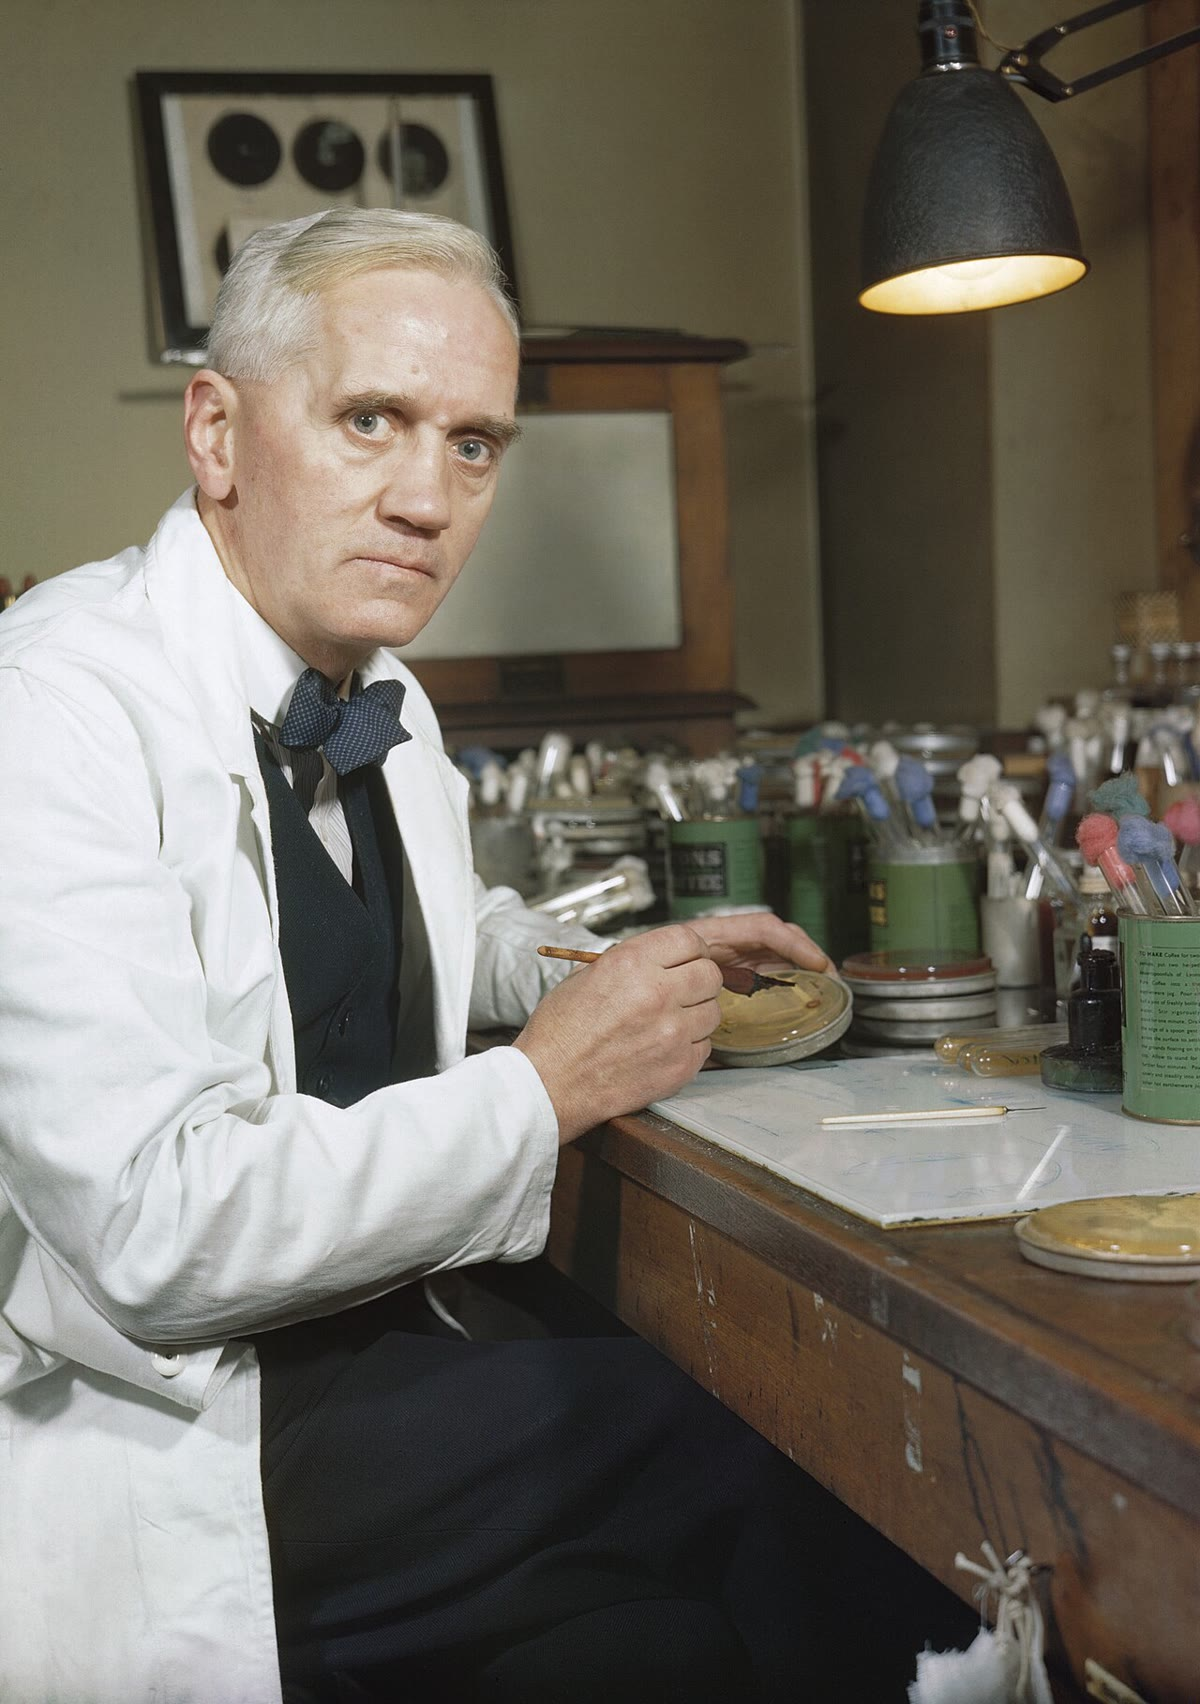
\includegraphics[width=0.4\linewidth]{images/book2/fleming.jpg}

{\small 1943 年，弗莱明在实验台前，身旁是十五年前他曾发现霉菌清除周围细菌的培养皿。照片：Imperial War Museums，公有领域。}
\end{omfigure}

\section{细菌如何变异}

\begin{proposition}[细菌的繁殖与变异]\label{prop:g11:antibiotic-resistance:variation}
细菌在复制其单个\omterm{def:g11:cell-cycle-mitosis:chromosome}{染色体}之后一分为二进行繁殖，
子代除复制错误外，在遗传上与母体相同，
即一个\emph{克隆}。在营养丰富的培养基中，
每 20 分钟分裂一次，10 小时内可使一个\omterm{def:g10:cells-common-unit:cell}{细胞}变为十亿个。
克隆内的遗传变异有两个来源：
\begin{itemize}
  \item \emph{\omterm{def:g11:mutations:mutation}{突变}}（见\cref{ch:g11:mutations}），每次分裂中罕见，
        但在数十亿个体的种群中很常见；
  \item \emph{基因水平转移}\index{基因水平转移}：
        从另一细菌获得的 \omterm{def:g10:universal-dna:information}{DNA}，可来自同种或异种细菌，
        最常见的形式是\emph{质粒}——一个小环状
        \omterm{def:g10:universal-dna:information}{DNA}，独立于\omterm{def:g11:cell-cycle-mitosis:chromosome}{染色体}之外，携带少量\omterm{def:g10:universal-dna:gene}{基因}，
        可经由膜桥在\omterm{def:g10:cells-common-unit:cell}{细胞}间传递。
\end{itemize}
\end{proposition}
\admitted

\begin{omfigure}
\begin{tikzpicture}[font=\small, >=Stealth]
  % donor
  \draw[thick, fill=omDef!10, rounded corners=12pt] (0,0) rectangle (3,1.5);
  \draw[thick, omDef] (0.4,0.75) .. controls (0.6,1.3) and (2.4,1.3) .. (2.6,0.75) .. controls (2.4,0.2) and (0.6,0.2) .. (0.4,0.75);
  \draw[thick, omThm, fill=omThm!20] (2.2,1.15) circle (0.22);
  \node[anchor=north] at (1.5,-0.1) {供体：含质粒};
  % recipient
  \draw[thick, fill=omDef!10, rounded corners=12pt] (5,0) rectangle (8,1.5);
  \draw[thick, omDef] (5.4,0.75) .. controls (5.6,1.3) and (7.4,1.3) .. (7.6,0.75) .. controls (7.4,0.2) and (5.6,0.2) .. (5.4,0.75);
  \node[anchor=north] at (6.5,-0.1) {受体};
  % bridge
  \draw[thick, fill=omProp!30] (3,0.55) rectangle (5,0.95);
  \draw[->, thick, omThm] (3.1,0.75) -- (4.9,0.75);
  \node[anchor=north, font=\scriptsize] at (4,-0.6) {质粒的一个副本穿过桥};
  % result
  \draw[->, thick] (8.4,0.75) -- (9.2,0.75);
  \draw[thick, fill=omDef!10, rounded corners=12pt] (9.5,0) rectangle (12.5,1.5);
  \draw[thick, omDef] (9.9,0.75) .. controls (10.1,1.3) and (11.9,1.3) .. (12.1,0.75) .. controls (11.9,0.2) and (10.1,0.2) .. (9.9,0.75);
  \draw[thick, omThm, fill=omThm!20] (11.7,1.15) circle (0.22);
  \node[anchor=north, align=center] at (11,-0.1) {受体现携带 \\ 质粒上的基因};
  \node[anchor=west, font=\scriptsize, omDef] at (0.2,1.75) {染色体};
  \node[anchor=west, font=\scriptsize, omThm] at (2.5,1.75) {质粒};
\end{tikzpicture}

{\small 水平转移。质粒是一种小环状 \omterm{def:g10:universal-dna:information}{DNA}，
可携带耐药\omterm{def:g10:universal-dna:gene}{基因}——经桥由一个细菌
复制到另一个细菌，二者不必是同一\omterm{def:g10:biodiversity-scales:species}{物种}。
受体及其所有后代一步即获得该\omterm{def:g10:universal-dna:gene}{基因}。}
\end{omfigure}

\begin{example}[种群中的计算]\label{ex:g11:antibiotic-resistance:arithmetic}
耐药\omterm{def:g11:mutations:mutation}{突变}约每 $10^8$ 次分裂出现一次。一瓶
含 $10^9$ 个细菌的培养物，在产生它的分裂过程中，
约出现十次此类\omterm{def:g11:mutations:mutation}{突变}；一处感染伤口或肠道，含 $10^{12}$
个细菌，约有一万次此类\omterm{def:g11:mutations:mutation}{突变}。每一个大型细菌种群
在使用\omterm{def:g11:antibiotic-resistance:antibiotic}{抗生素}之前就含有对其耐药的\omterm{def:g10:cells-common-unit:cell}{细胞}——
在\cref{ch:g11:mutations}中，影印平板已证实了这一点。
\end{example}

\section{抗生素}

\begin{definition}[抗生素]\label{def:g11:antibiotic-resistance:antibiotic}
称\emph{抗生素}\index{抗生素}为一种分子，能杀死
细菌或抑制其生长，在对患者\omterm{def:g10:cells-common-unit:cell}{细胞}无害的浓度下，
通过作用于细菌具有而人类\omterm{def:g10:cells-common-unit:cell}{细胞}不具有的结构或过程
实现杀菌：青霉素及其同类物阻断
细菌\omterm{def:g10:cells-common-unit:organelle}{细胞壁}的合成；链霉素和四环素干扰
细菌\omterm{def:g10:cells-common-unit:organelle}{核糖体}，其结构与人体的不同；其他药物阻断
细菌中参与 \omterm{def:g10:universal-dna:information}{DNA} 复制的酶。多数抗生素最初发现于
霉菌和土壤细菌中，它们借此对抗竞争者。
抗生素对病毒无效，因为病毒不具有这些
作用靶点。
\end{definition}

\begin{proposition}[耐药机制]\label{prop:g11:antibiotic-resistance:mechanisms}
若细菌对某种\omterm{def:g11:antibiotic-resistance:antibiotic}{抗生素}\emph{耐药}\index{抗生素耐药性}，即它能在
足以抑制其敏感同类的浓度下生长。耐药性的遗传基础有几类之一：
同类。耐药性的遗传基础属于以下几类之一：
一种\omterm{def:g10:universal-dna:gene}{基因}编码能破坏\omterm{def:g11:antibiotic-resistance:antibiotic}{抗生素}的酶（青霉素酶可将
青霉素断为两段）；一种\omterm{def:g11:mutations:mutation}{突变}改变\omterm{def:g11:antibiotic-resistance:antibiotic}{抗生素}的靶点，
使药物不再结合（\omterm{def:g10:cells-common-unit:organelle}{核糖体}蛋白发生改变）；一种泵
将药物排出；一种壁使药物无法进入。每一种都是
一个\omterm{def:g10:universal-dna:gene}{等位基因}或\omterm{def:g10:universal-dna:gene}{基因}，且均可遗传——在克隆内垂直传递，
若位于质粒上，则可在邻近细菌间水平传递。
\end{proposition}
\admitted

\begin{method}[读取药敏试验结果]\label{met:g11:antibiotic-resistance:antibiogram}
\emph{药敏试验}可同时用
多种\omterm{def:g11:antibiotic-resistance:antibiotic}{抗生素}检测患者的细菌。
\begin{enumerate}
  \item 将细菌均匀涂布于平板上；放置
        各浸有一种\omterm{def:g11:antibiotic-resistance:antibiotic}{抗生素}的纸片；过夜培养。
  \item \omterm{def:g11:antibiotic-resistance:antibiotic}{抗生素}从纸片中扩散出来，其浓度
        随距离增加而降低；细菌长成一片菌苔，
        仅在浓度足以抑制它们处，形成透明的\emph{抑菌圈}，
        环绕每张纸片。
  \item 测量每个抑菌圈的直径，与该\omterm{def:g11:antibiotic-resistance:antibiotic}{抗生素}
        规定的阈值比较：直径大于阈值
        为敏感，小于阈值则为耐药。
  \item 在敏感结果中，抑菌圈最大者
        为用药提供依据；纸片周围完全无抑菌圈的，
        即该菌株不受其抑制的\omterm{def:g11:antibiotic-resistance:antibiotic}{抗生素}。
\end{enumerate}
\end{method}

\begin{omfigure}
\begin{tikzpicture}[font=\small]
  \draw[thick, fill=omProp!12] (0,0) circle (3.7);
  \foreach \a/\r/\l in {90/1.3/A, 162/0.9/B, 234/0.0/C, 306/1.6/D, 18/0.55/E} {
    \begin{scope}[shift={(\a:2.0)}]
      \ifdim \r pt > 0pt \draw[fill=white] (0,0) circle (\r); \fi
      \draw[fill=gray!30] (0,0) circle (0.28);
      \node[font=\scriptsize] at (0,0) {\l};
    \end{scope}
  }
  \node[anchor=west, align=left] at (3.8,1.6) {A：抑菌圈 \qty{26}{mm}，阈值 17：敏感};
  \node[anchor=west, align=left] at (3.8,0.9) {B：抑菌圈 \qty{18}{mm}，阈值 20：耐药};
  \node[anchor=west, align=left] at (3.8,0.2) {C：无抑菌圈，耐药};
  \node[anchor=west, align=left] at (3.8,-0.5) {D：抑菌圈 \qty{32}{mm}，阈值 22：敏感};
  \node[anchor=west, align=left] at (3.8,-1.2) {E：抑菌圈 \qty{11}{mm}，阈值 15：耐药};
  \node[anchor=north, align=center] at (0,-3.9) {患者细菌的菌苔；\\ 每张纸片周围的透明抑菌圈};
\end{tikzpicture}

{\small 药敏试验结果的读法。每张纸片含一种\omterm{def:g11:antibiotic-resistance:antibiotic}{抗生素}，透明
区域即细菌无法生长之处。将各抑菌圈直径与对应药物阈值比较后，
可判定该菌株对 A 与 D 敏感，
对 B、C 和 E 耐药。}
\end{omfigure}

\begin{omfigure}
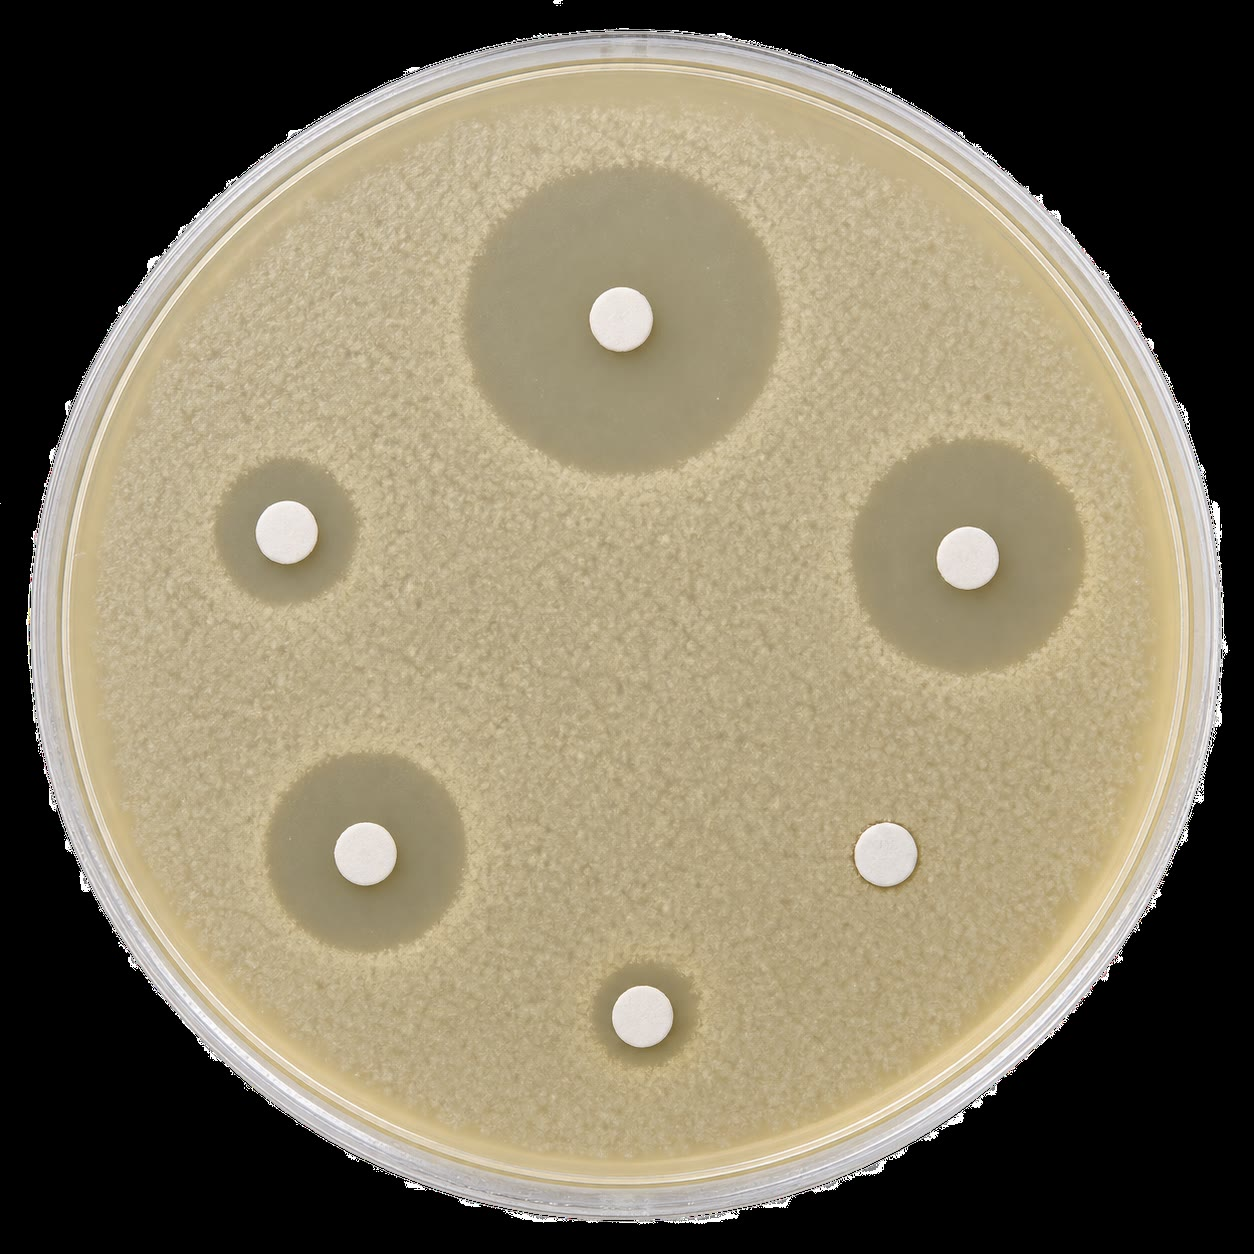
\includegraphics[width=0.44\linewidth]{images/book2/ai/g11-antibiogram-plate.jpg}

{\small 过夜培养后的药敏试验平板：一层细菌菌苔，
每张\omterm{def:g11:antibiotic-resistance:antibiotic}{抗生素}纸片周围有一个透明抑菌圈，其大小
反映该菌株的敏感程度。有一张纸片周围无抑菌圈。}
\end{omfigure}

\section{耐药性如何传播}

\begin{proposition}[抗生素的选择作用]\label{prop:g11:antibiotic-resistance:selection}
\omterm{def:g11:antibiotic-resistance:antibiotic}{抗生素}并不产生耐药细菌，而是\emph{选择}
它们。若种群中少数\omterm{def:g10:cells-common-unit:cell}{细胞}携带耐药\omterm{def:g10:universal-dna:gene}{等位基因}，
药物杀死或抑制多数敏感\omterm{def:g10:cells-common-unit:cell}{细胞}，使少数
耐药\omterm{def:g10:cells-common-unit:cell}{细胞}无竞争地增殖：数日内，该
种群即转为耐药。\omterm{def:g11:antibiotic-resistance:antibiotic}{抗生素}用得越多——无论是
用于患者、动物还是环境中——这种
选择发生得越频繁，医院、农场或一个国家的细菌
便越耐药。疗程不完整，杀死最敏感的\omterm{def:g10:cells-common-unit:cell}{细胞}、
留下的敏感\omterm{def:g10:cells-common-unit:cell}{细胞}最少，选择效率最高。
\end{proposition}
\begin{proof}[证据]
莱德伯格的影印平板表明，耐药\omterm{def:g10:cells-common-unit:cell}{细胞}在接触药物之前
就已存在。在浓度递增的\omterm{def:g11:antibiotic-resistance:antibiotic}{抗生素}中培养一周的菌群，
最终对初始剂量的一百倍仍具耐药性，
且耐药性可遗传，并定位到特定\omterm{def:g11:mutations:mutation}{突变}。
人均\omterm{def:g11:antibiotic-resistance:antibiotic}{抗生素}用量最高的国家，耐药菌株
所占比例也最高；减少用药的医院病房，
耐药性数月内即会下降。皮肤细菌的一株
\emph{Staphylococcus aureus}对青霉素耐药的菌株，
在该药投入使用后四年内出现，现已占医院菌株的大多数；
对替代药物耐药的菌株，
则在替代药物推出两年后出现。
\end{proof}

\begin{omfigure}
\begin{tikzpicture}
\begin{axis}[
  width=0.88\linewidth, height=5.8cm,
  axis x line=bottom, axis y line=left,
  xmin=0, xmax=6, ymin=0, ymax=110,
  xlabel={用药天数}, ylabel={细菌（占初始量 \%）},
  xlabel style={font=\small, at={(axis description cs:0.5,-0.12)}, anchor=north},
  ylabel style={font=\small},
  tick label style={font=\small}, xtick={0,1,2,3,4,5,6}, ytick={0,25,50,75,100},
  legend style={at={(0.5,-0.3)}, anchor=north, legend columns=3, font=\small, draw=none},
  clip=false,
]
\addplot[thick, omDef] coordinates {(0,100) (0.5,45) (1,15) (1.5,5) (2,1.5) (3,0.2) (4,0.05) (5,0.01) (6,0)};
\addplot[thick, omThm] coordinates {(0,0.001) (1,0.01) (2,0.1) (3,1) (4,8) (5,40) (6,100)};
\addplot[thick, omMeth, dashed] coordinates {(0,100) (0.5,45) (1,15) (1.5,5) (2,1.5) (3,1.2) (4,9) (5,48) (6,100)};
\legend{敏感细胞, 耐药细胞（初始为 $10^5$ 个之一）, 第 3 天停药时的总数}
\end{axis}
\end{tikzpicture}

{\small \omterm{def:g11:antibiotic-resistance:antibiotic}{抗生素}疗程中的选择作用。敏感\omterm{def:g10:cells-common-unit:cell}{细胞}
（蓝色）数日内被杀死；少数耐药\omterm{def:g10:cells-common-unit:cell}{细胞}（红色）
无对抗地增殖，到一周末时占据整个种群。
若患者在第 3 天停药，幸存者重新生长——此时几乎全部
为耐药\omterm{def:g10:cells-common-unit:cell}{细胞}。}
\end{omfigure}

\begin{example}[从一个细胞到一间病房]\label{ex:g11:antibiotic-resistance:ward}
一名接受青霉素治疗的患者体内，在 $10^{10}$ 个细菌中，
带有一百个耐药细菌。三天之内，敏感细菌消失殆尽，
耐药克隆取而代之，数量达 $10^{10}$ 个耐药\omterm{def:g10:cells-common-unit:cell}{细胞}。
\omterm{def:g10:cells-common-unit:cell}{细胞}。这一克隆可存在于护士的手上、床栏上，或下一位患者体内，
克隆继续扩散——若其耐药\omterm{def:g10:universal-dna:gene}{基因}位于质粒上，它
便会沿途将其传给其他\omterm{def:g10:biodiversity-scales:species}{物种}。整个过程中，
\omterm{def:g11:antibiotic-resistance:antibiotic}{抗生素}无须作用于 \omterm{def:g10:universal-dna:information}{DNA}，它只是清除了
竞争对手。
\end{example}

\section{保持抗生素有效}

\begin{proposition}[后果与应对]\label{prop:g11:antibiotic-resistance:consequences}
耐药感染病程更长、费用更高，致死率也更高；
部分菌株如今对所有可用药物均有耐药性。由于耐药性
由用药所驱动，应对之策是少用、善用\omterm{def:g11:antibiotic-resistance:antibiotic}{抗生素}：
仅用于细菌感染（切勿用于病毒性感冒和流感），
条件允许时，依据药敏试验结果选药，足量
足疗程用药，选用有效的最窄谱药物；限制其在养殖业中的使用；
预防感染（注意卫生、接种疫苗），以减少
所需疗程；并在医院中隔离耐药菌株的携带者。
新药只能争取时间；选择的规律决定了
每一种新药终将出现耐药性。
\end{proposition}
\admitted

\begin{remark}[一周之内的演化]\label{rem:g11:antibiotic-resistance:evolution}
\omterm{def:g11:mutations:mutation}{突变}随机提供变异，环境对其进行筛选，
幸存者的后代继承这一差异：本章的
细菌在一周之内走完了
末章将用数百万年、以鲸和橡树为例描述的过程。
\omterm{def:g11:antibiotic-resistance:antibiotic}{抗生素}耐药性是在真实时间中观察到的
自然选择式演化，人类是选择的施加者——也是
最清楚的证明：这一过程并非关于过去的理论，而是
对任何能变异、能繁殖的种群都成立的事实。
\end{remark}

\section{练习}

\begin{exercise}[$\star$]\label{exo:g11:antibiotic-resistance:1}
说出细菌种群中遗传变异的两个来源。
\end{exercise}

\begin{exercise}[$\star$]\label{exo:g11:antibiotic-resistance:2}
什么是\omterm{def:g11:antibiotic-resistance:antibiotic}{抗生素}？它为何能伤害细菌而不伤害
患者的\omterm{def:g10:cells-common-unit:cell}{细胞}？为什么它对感冒无效？
\end{exercise}

\begin{exercise}[$\star$]\label{exo:g11:antibiotic-resistance:3}
给出细菌抵抗\omterm{def:g11:antibiotic-resistance:antibiotic}{抗生素}的三种机制。
\end{exercise}

\begin{exercise}[$\star$]\label{exo:g11:antibiotic-resistance:4}
在药敏图中，新纸片 F 形成的
抑菌圈为 \qty{20}{mm}，阈值为 \qty{18}{mm}。该菌株是敏感还是
耐药？在 A 至 F 中你会选用哪种\omterm{def:g11:antibiotic-resistance:antibiotic}{抗生素}？
\end{exercise}

\begin{exercise}[$\star$]\label{exo:g11:antibiotic-resistance:5}
\omterm{def:g11:antibiotic-resistance:antibiotic}{抗生素}会导致耐药性\omterm{def:g11:mutations:mutation}{突变}吗？请结合
\cref{ch:g11:mutations}中的实验加以论证。
\end{exercise}

\begin{exercise}[$\star\star$]\label{exo:g11:antibiotic-resistance:6}
从一个每 20 分钟分裂一次的细菌开始，
10 小时后共有多少个细菌？若每 $10^8$ 次分裂
出现一次耐药性，培养物中可能含有多少耐药\omterm{def:g10:cells-common-unit:cell}{细胞}？
\end{exercise}

\begin{exercise}[$\star\star$]\label{exo:g11:antibiotic-resistance:7}
由选择图可知，耐药\omterm{def:g10:cells-common-unit:cell}{细胞}在哪一天成为
总数中的多数？在虚线所示情形下，第 6 天的
种群总数是多少？它由哪些\omterm{def:g10:cells-common-unit:cell}{细胞}组成？
\end{exercise}

\begin{exercise}[$\star\star$]\label{exo:g11:antibiotic-resistance:8}
解释为什么位于质粒上的耐药\omterm{def:g10:universal-dna:gene}{基因}比位于
\omterm{def:g11:cell-cycle-mitosis:chromosome}{染色体}上的传播得更快。
\end{exercise}

\begin{exercise}[$\star\star$]\label{exo:g11:antibiotic-resistance:9}
一位患者服用三天、疗程为七天的药后感觉好转，便
停药。请结合图示说明之后几天会发生什么，
以及为什么复发更难治疗。
\end{exercise}

\begin{exercise}[$\star\star$]\label{exo:g11:antibiotic-resistance:10}
为什么医院中耐药菌株的比例高于
普通人群？
\end{exercise}

\begin{exercise}[$\star\star$]\label{exo:g11:antibiotic-resistance:11}
解释为什么改变\omterm{def:g10:cells-common-unit:organelle}{核糖体}蛋白的\omterm{def:g11:mutations:mutation}{突变}可使
细菌对链霉素产生耐药性，以及这类细菌为何往往
比敏感的近缘菌株生长得稍慢。
\end{exercise}

\begin{exercise}[$\star\star\star$]\label{exo:g11:antibiotic-resistance:12}
两种作用靶点不同的\omterm{def:g11:antibiotic-resistance:antibiotic}{抗生素}联合使用。估计
某\omterm{def:g10:cells-common-unit:cell}{细胞}因两次独立\omterm{def:g11:mutations:mutation}{突变}（各为 $10^8$ 分之一）
而对两者同时耐药的概率，并说明为什么
对结核病这类缓慢、持续时间长的感染要采用联合疗法。
\end{exercise}

\begin{exercise}[$\star\star\star$]\label{exo:g11:antibiotic-resistance:13}
某农场在动物饲料中添加低剂量\omterm{def:g11:antibiotic-resistance:antibiotic}{抗生素}，以促进
动物生长。请预测其对动物体内细菌、
农场工人以及人类医疗的影响，
并运用选择和水平\omterm{def:g10:universal-dna:gene}{基因}转移加以说明。
\end{exercise}

\begin{exercise}[$\star\star\star$]\label{exo:g11:antibiotic-resistance:14}
某病房将\omterm{def:g11:antibiotic-resistance:antibiotic}{抗生素}处方减半；一年之内，
耐药菌株的比例下降。请解释耐药性
为何会消退，并运用耐药性对细菌的代价
以及竞争加以说明。
\end{exercise}

\begin{exercise}[$\star\star\star$]\label{exo:g11:antibiotic-resistance:15}
“细菌产生耐药性，是因为它们对\omterm{def:g11:antibiotic-resistance:antibiotic}{抗生素}产生了适应。”
请用\omterm{def:g11:mutations:mutation}{突变}、选择和遗传，在一小段文字中
正确改写这句话。
\end{exercise}

\section{问题：病房}

\begin{problem}[{周末问题——一次医院病房的暴发
源于单个突变细胞：菌落的计算、
药敏图的判读、疗程的中断，以及阻止
扩散的策略}]
\label{pb:g11:antibiotic-resistance:1}
某患者伤口感染了 $10^{10}$ 个同种细菌。
这些细菌每 30 分钟分裂一次；产生对阿莫西林耐药性的
\omterm{def:g11:mutations:mutation}{突变}每 $10^8$ 次分裂出现一次。
该\omterm{def:g11:antibiotic-resistance:antibiotic}{抗生素}每 6 小时杀死 90\% 的敏感\omterm{def:g10:cells-common-unit:cell}{细胞}，
对耐药\omterm{def:g10:cells-common-unit:cell}{细胞}没有影响，耐药\omterm{def:g10:cells-common-unit:cell}{细胞}继续分裂。

\medskip
\noindent\textbf{第一部分——治疗前。}
\begin{enumerate}
  \item 第一个\omterm{def:g10:cells-common-unit:cell}{细胞}经过多少次分裂，产生了 $10^{10}$ 个细菌？
        （数一数\omterm{def:g10:cells-common-unit:cell}{细胞}的个数。）
  \item 估计在使用任何\omterm{def:g11:antibiotic-resistance:antibiotic}{抗生素}之前，
        已存在的耐药\omterm{def:g10:cells-common-unit:cell}{细胞}数。
  \item 解释为何患者的感染在药敏图上仍被描述为
        “敏感”。
  \item 药敏图显示，阿莫西林的抑菌圈为 \qty{24}{mm}（阈值 17），
        红霉素的抑菌圈为 \qty{12}{mm}（阈值 20），
        青霉素无抑菌圈。请解释这三项结果。
  \item 医生开具阿莫西林，疗程为 \num{7}~天。为何不用青霉素，
        以及若另一种药的抑菌圈更大，
        为何不选抑菌圈最大的药物？
\end{enumerate}

\medskip
\noindent\textbf{第二部分——治疗期间。}
\begin{enumerate}[resume]
  \item 经过 \num{1}~天后还剩多少个敏感\omterm{def:g10:cells-common-unit:cell}{细胞}？经过 \num{3}~天后呢？
  \item 以第 2 题的答案为起点，若耐药\omterm{def:g10:cells-common-unit:cell}{细胞}每 30 分钟加倍一次且不受限制，
        则 \num{1}~天后会有多少个耐药\omterm{def:g10:cells-common-unit:cell}{细胞}？
        （取 $2^{48} \approx \num{2.8e14}$。）为何这一数值不现实？
        又是什么限制了它的增长？
  \item 假设耐药克隆只能占据敏感\omterm{def:g10:cells-common-unit:cell}{细胞}让出的空间，
        因而其数量不超过 $10^{10}$。
        大约何时会充满这一空间？
  \item 画出或描述敏感\omterm{def:g10:cells-common-unit:cell}{细胞}、耐药\omterm{def:g10:cells-common-unit:cell}{细胞}和细菌总数
        在 \num{7}~天内的变化曲线。
  \item 实际上，患者的免疫系统会在数天内清除最后剩下的
        几百万个任何类型的\omterm{def:g10:cells-common-unit:cell}{细胞}。试解释结果为何取决于
        耐药克隆的增长速度是否快于
        免疫系统清除它的速度。
\end{enumerate}

\medskip
\noindent\textbf{第三部分——疗程中断。}
\begin{enumerate}[resume]
  \item 患者用药 \num{2}~天后感觉良好，遂停止服药。此时还剩多少个敏感\omterm{def:g10:cells-common-unit:cell}{细胞}，
        幸存群体中耐药\omterm{def:g10:cells-common-unit:cell}{细胞}所占的比例
        是多少？
  \item 此后数日内，细菌数量回升至 $10^{10}$。
        若耐药\omterm{def:g10:cells-common-unit:cell}{细胞}与敏感\omterm{def:g10:cells-common-unit:cell}{细胞}的增殖速率相同，
        则现在耐药\omterm{def:g10:cells-common-unit:cell}{细胞}占多大比例？
  \item 患者复发，再次使用阿莫西林治疗，
        试预测其结果。
  \item 复发时的药敏图显示阿莫西林无抑菌圈。
        试解释它与第一次药敏图相比为何发生了变化。
  \item 耐药\omterm{def:g10:universal-dna:gene}{基因}位于质粒上，这会为病房带来
        哪些额外风险？
\end{enumerate}

\medskip
\noindent\textbf{第四部分——病房的管理策略。}
病房每年用阿莫西林治疗 400 名患者；病房内分离的感染
菌株中有 30\% 现已耐药，
而全镇的这一比例仅为 5\%。
\begin{enumerate}[resume]
  \item 试从选择压力的角度解释病房与全镇之间
        的差异。
  \item 病房作出以下决定：每次开药前先检测药敏图，
        完成全部疗程、勤洗手，并隔离耐药菌株的携带者。
        请说明每项措施分别作用于
        本章中的哪一种机制。
  \item 两年后，病房内的耐药率降至 12\%。试解释它为何下降，
        以及为何未能回落到 5\%。
  \item 为何在病房引入的一种新\omterm{def:g11:antibiotic-resistance:antibiotic}{抗生素}，
        也无法在几年以上的时间内解决问题？
  \item 请给出结论：伤口在用药前所含的耐药\omterm{def:g10:cells-common-unit:cell}{细胞}数、
        这些耐药\omterm{def:g10:cells-common-unit:cell}{细胞}获得耐药性的那一天，
        以及使一种可治愈的感染演变为暴发的、
        患者的那一个单一习惯。
\end{enumerate}
\end{problem}
